\documentclass[twoside,10pt,letterpaper]{refart}
\usepackage{ifthen}
\usepackage[colorlinks=true,citecolor=blue,linkcolor=blue]{hyperref}
\usepackage{bytefield}
\usepackage{makeidx}
\usepackage[T1]{fontenc}
\usepackage[lining]{ebgaramond}
\usepackage{tikz}
\usetikzlibrary{shapes.geometric, arrows}

\usepackage{fontspec}
\setmonofont{Courier Prime}

\newfontfamily\codefamily{BigBlue}
\DeclareTextFontCommand{\codefont}{\codefamily}

\newcommand{\forceindent}[1][3em]{\leavevmode{\parindent=#1\indent}}

% facilitates the creation of memory maps. Start address at the bottom, end address at the top.
% syntax: \memsection{end address}{start address}{height in lines}{text in box}
% source: https://www.martin-demling.de/2011/06/memory-maps-in-latex-using-the-bytefield-package/
\newcommand{\memsection}[4]{
    \bytefieldsetup{bitheight=#3\baselineskip}    % define the height of the memsection
    \bitbox[]{10}{
        \texttt{#1}     % print end address
        \\ \vspace{#3\baselineskip} \vspace{-2\baselineskip} \vspace{-#3pt} % do some spacing
        \texttt{#2}     % print start address
    }
    \bitbox{16}{#4} % print box with caption
}

\ExplSyntaxOn
\cs_new:Npn \m88 {
    {\codefamily M88}
}
\ExplSyntaxOff
\newcommand{\itwoc}{I\textsuperscript{2}C}

\tikzstyle{startstop} = [rectangle, rounded corners, minimum width=3cm, minimum height=1cm,text centered, text width=3cm, draw=black]
\tikzstyle{io} = [trapezium, trapezium left angle=70, trapezium right angle=110, minimum width=3cm, minimum height=1cm, text centered, text width=3cm, draw=black]
\tikzstyle{process} = [rectangle, minimum width=3cm, minimum height=1cm, text centered, text width=3cm, draw=black]
\tikzstyle{decision} = [diamond, minimum width=3cm, minimum height=1cm, text centered, text width=3cm, aspect=3, draw=black]
\tikzstyle{arrow} = [thick,->,>=stealth]

\makeindex

\title{The \m88 Computer Manual}
\author{Matthew Iselin}
\date{}

\fullpage


\begin{document}
\maketitle
\raggedright
\footnotesize

\tableofcontents

\newpage

\part{The \m88 Computer}

\section{What is the \m88 Computer?}
The \m88 Computer is a computer designed around the Intel 8088 processor.
It is loosely based on the IBM PC, but with a few modern touches and simplifications
to make it easier to build and understand.

The computer was designed with a single goal in mind: to run Sid Meier's Civilization.
I achieved that goal, and now I'm sharing the design with the world.

\section{Getting Started}
The \m88 Computer is optimized for production using \href{https://jlcpcb.com}{JLCPCB's}
PCB Assembly services and \href{https://lcsc.com}{LCSC's} component sourcing. For this reason,
many of the passive components are surface-mount rather than through-hole. Even so, it is
possible to hand-solder the motherboard if you are so inclined.

Because the design is optimized for PCB assembly, values are not annotated on the silkscreen.
It is recommended to keep the motherboard's KiCad project close by to verify values and connections.
You can obtain the KiCad files from the project GitHub repository at \url{https://github.com/miselin/M88}.

A fully assembled PCB will include DIP sockets for all ICs, and all other components will be
present (including ISA slots and PS/2 ports). You will need to populate the board with the
required ICs. A system ROM is required and can be downloaded from the same GitHub repository.

The ATTiny system management controller will also need to be programmed.

\section{Required ICs}
The \m88 Computer requires the following ICs:
\begin{itemize}
    \item 2x Intel 8284 clock generator
    \item 3x 74LS573 or equivalent
    \item 1x 74LS688 or 74F521
    \item 1x 7406
    \item 1x 75477
    \item 1x Intel 8088 processor, or equivalent (e.g. NEC V20)
    \item 2x 74LS125
    \item 1x 74LS244
    \item 1x 74LS32
    \item 1x 74HC245
    \item 1x 74LS175
    \item 1x 74LS04
    \item 2x Intel 8259 Programmable Interrupt Controller
    \item 2x 74LS247
    \item 1x Intel 8254 Programmable Interval Timer
    \item 3x 72LS138
    \item 1x 74LS02
    \item 1x 74HC74
    \item 1x 74LS00
    \item 1x 74LS08
    \item 1x ATTiny13A
    \item 1x W27C512 EEPROM
    \item 1-5x AS6C1008-55PCN SRAM
    \item 1x VIA VT82C42 PS/2 Controller
\end{itemize}

You may use HCT or ACT series chips instead of LS series chips, but the design has not
been tested with them. If the motherboard was not pre-populated with crystals, you will
also need one 24 MHz crystal and one 14.31818 MHz crystal. You may experiment with the
value of the 24 MHz crystal. The system may not operate correctly if the 14.31818 MHz
crystal value is changed, as this drives time-keeping and the ISA bus clock.

\subsubsection{Crystal Selection}
The default crystals of 24 MHz and 14.31818 MHz provide a CPU clock of 8 MHZ and an ISA
bus clock of 14.31818 MHz.

Generally, it is not recommended to change the 14.31818 MHz crystal, as this drives the
ISA bus and Programmable Interval Timer. Changing its frequency may require software changes
to handle the different clock.

The 24 MHz crystal can be changed to provide a different CPU clock. The CPU operates at
1/3 the crystal frequency.

\section{Required Peripherals}
To use the \m88 Computer, you will need the following:
\begin{itemize}
    \item A Micro-ATX case is \emph{strongly} recommended for grounding
    \item An ATX power supply
    \item An 8-bit ISA VGA card. The computer has been extensively tested with a Trident TVGA8900C.
    \item An 8-bit ISA storage controller. The computer has been tested with an XT-IDE.
    \item A PS/2 keyboard
\end{itemize}

\section{Features}
\begin{itemize}
    \item Built around the Intel 8088 processor, clocked at 8 MHz
    \item Up to 640 KiB of conventional RAM, using SRAM instead of traditional DRAM
    \item Four 8-bit ISA slots
    \item 2 PS/2 ports
    \item PC Speaker socket
    \item On-board 7-segment POST code display
    \item A Micro-ATX form factor motherboard for easy integration into modern cases
    \item ATTiny-based system manager to handle reset and ATX power supply control
    \item ATX fan headers for cooling
\end{itemize}

\section{Differences from the IBM PC}
The \m88 Computer is not a 100\% clone of the IBM PC. It is missing a
DMA controller, which limits the ability to use certain peripherals. The lack of a
DMA controller is an intentional simplification.

The \m88 Computer uses SRAM instead of DRAM for the main memory. This
further simplifies the design, but also makes it more expensive.

The \m88 Computer adds the second 8259 interrupt controller, which was
not present in the original IBM PC. This allows for more interrupts to be used,
in particular IRQ \#12 which is used by PS/2 mice.

\newpage

\section{I/O Map}

\begin{center}
\begin{bytefield}{24}
    \memsection{FFFF}{0100}{6}{Available for Peripherals}\\
    \memsection{00FF}{00B0}{4}{Reserved}\\
    \memsection{00AF}{00A0}{3}{8259 Interrupt Controller (Secondary)}\\
    \memsection{009F}{0090}{3}{Reserved}\\
    \memsection{008F}{0080}{3}{POST Codes}\\
    \memsection{007F}{0050}{4}{Reserved}\\
	\memsection{004F}{0040}{3}{8254 Programmable Interval Controller}\\
    \memsection{003F}{0030}{3}{Reserved}\\
	\memsection{002F}{0020}{3}{8259 Interrupt Controller (Primary)}\\
	\memsection{001F}{0000}{3}{Reserved}\\
\end{bytefield}
\end{center}

\newpage

\section{Memory Map}

The \m88 Computer has a maximum of 640 KiB of conventional memory. At
least one SRAM chip is required in Slot \#1 to provide the first 64 KiB of memory.
SRAM should be loaded in sequential slots. "Skipping" a slot will result in the system
reporting less available memory than is actually installed.

The recommended SRAM chip is the \texttt{AS6C1008-55PCN}, but any pin-compatible 128 KiB SRAM
chips can be used.

The memory map for the \m88 Computer is as follows:

\begin{center}
\begin{bytefield}{24}
    \memsection{FFFF:FFFF}{F000:0000}{3}{System BIOS}\\
    \memsection{EFFF:FFFF}{A000:0000}{6}{Available for Option ROMs and Peripheral Memory}\\
    \begin{rightwordgroup}{Conventional Memory}
    \memsection{9FFF:FFFF}{8000:0000}{3}{System RAM Slot \#5}\\
    \memsection{7FFF:FFFF}{6000:0000}{3}{System RAM Slot \#4}\\
    \memsection{5FFF:FFFF}{4000:0000}{3}{System RAM Slot \#3}\\
    \memsection{3FFF:FFFF}{2000:0000}{3}{System RAM Slot \#2}\\
    \memsection{1FFF:FFFF}{0000:0000}{3}{System RAM Slot \#1}
    \end{rightwordgroup}\\
\end{bytefield}
\end{center}

\newpage

\section{Troubleshooting}
If the system does not boot, the POST code display will show a two-digit code.
See below for a list of POST codes and what they mean.

\begin{center}
\begin{tabular}{ c|c }
 \texttt{00} & BIOS code has started to run \\\hline
 \texttt{01} & CPU registers are OK \\\hline
 \texttt{02} & First 64K of memory is OK \\\hline
 \texttt{03} & Interrupt handlers installed \\\hline
 \texttt{04} & Programmable interrupt controller configured \\\hline
 \texttt{05} & Programmable interval controller configured \\\hline
 \emph{<<beep>>} & \emph{see above} \\\hline
 \texttt{06} & CPU interrupts enabled \\\hline
 \texttt{07} & Video BIOS complete \\\hline
 \texttt{08} & Memory count complete \\\hline
 \texttt{09} & Stack relocated to top of conventional memory \\\hline
 \texttt{10} & Extended BIOS data area installed \\\hline
 \texttt{11} & PS/2 controller configured \\\hline
 \texttt{12} & Serial and Parallel ports configured (if present) \\\hline
 \texttt{88} & All Option ROMs successfully called, about to call INT19 \\
\end{tabular}
\end{center}

\section{Power Specifications}

Current draws are controlled by PTC resettable fuses. If the system is behaving erratically,
check the temperature of each PTC fuse. If a fuse is hot, it has tripped and is limiting current.
The system should be powered off until the fuse has cooled and reset, and the cause for the overcurrent
should be investigated.

\begin{center}
\begin{tabular}{ c|c|c  }
 \hline
 \textbf{Voltage Rail}   & \textbf{Max Current}    & \textbf{Purpose} \\
 \hline
 +5V & 2A & Main system power for all components. \\
 +5V PS/2 & 1A & PS/2 power, derived from +5V with its own fuse. \\
 +5V SB & 0.5A & Always-on standby power (for ATX power signaling). \\
 +12V & 1A & ISA bus power rail. \\
 -12V & 1A & ISA bus power rail. \\
\end{tabular}
\end{center}

\section{INT 88H: \m88 BIOS Services} \label{bios}
The \m88 BIOS provides a number of services to the system. These services are accessed through the \texttt{INT 88H}
software interrupt.

The value of the AX register, and any input registers, will not be preserved across \m88 BIOS calls. All other registers
will be preserved.

\subsection{Function 24H: Write \itwoc{} Byte}
\textbf{To call:}

\begin{tabular}{@{\hspace{2em}}l@{}l@{\hspace{2em}}l}
{} & AH & = 24H \\
{} & AL & = \itwoc{} device address \\
{} & BL & = \itwoc{} data byte \\[\parskip]
{} & \multicolumn{2}{@{}l}{\textit{\textbf{Note:}} This service will block until the \itwoc{} bus is idle.}
\end{tabular}

\textbf{Returns:}

\begin{tabular}{@{\hspace{2em}}l@{}l@{\hspace{2em}}l}
{} & \multicolumn{2}{@{}l}{Nothing}
\end{tabular}

\subsection{Function 25H: Read \itwoc{} Byte}
\textbf{To call:}

\begin{tabular}{@{\hspace{2em}}l@{}l@{\hspace{2em}}l}
{} & AH & = 54H \\
{} & AL & = \itwoc{} device address \\[\parskip]
{} & \multicolumn{2}{@{}l}{\textit{\textbf{Note:}} This service will block until the \itwoc{} bus is idle.}
\end{tabular}

\textbf{Returns:}

\begin{tabular}{@{\hspace{2em}}l@{}l@{\hspace{2em}}l}
{} & AL & = \itwoc{} data byte
\end{tabular}

\subsection{Function 26H: Check \itwoc{} Bus State}
\textbf{To call:}

\begin{tabular}{@{\hspace{2em}}l@{}l@{\hspace{2em}}l}
{} & AH & = 26H
\end{tabular}

\textbf{Returns:}

\begin{tabular}{@{\hspace{2em}}l@{}l@{\hspace{2em}}l}
{} & AL & = Zero if the \itwoc{} bus is idle, non-zero if busy.
\end{tabular}

\subsection{Function 27H: Set \itwoc{} Device Address}
\textbf{To call:}

\begin{tabular}{@{\hspace{2em}}l@{}l@{\hspace{2em}}l}
{} & AH & = 27H \\
{} & BL & = New \itwoc{} device address for the controller
\end{tabular}

\textbf{Returns:}

\begin{tabular}{@{\hspace{2em}}l@{}l@{\hspace{2em}}l}
{} & \multicolumn{2}{@{}l}{Nothing}
\end{tabular}

\newpage

\part{Peripherals}

\section{ISA-to-\itwoc{} Bridge}

\subsection{Introduction}
The ISA-to-\itwoc{} bridge is a simple device that allows the \m88 Computer to communicate
with \itwoc{} devices.

\subsection{Configuration}
The ISA-to-\itwoc{} bridge card includes a DIP switch to configure the I/O port address.
Ports in the range \texttt{0x00} to \texttt{0x3FF} can be configured. Your configuration needs may
vary depending on other peripherals installed on the system, but generally port \texttt{0x3A0} should
work.

Note that the DIP switch controls address bits 2 through 9, requiring the address to be aligned to
a 4-byte boundary.

The DIP switch positions for port \texttt{0x3A0} are as follows:

\begin{center}
    \begin{tabular}{ c|c|c|c|c|c|c|c|c }
        \textbf{DIP Switch} & A9 & A8 & A7 & A6 & A5 & A4 & A3 & A2 \\
        \hline
        \textbf{Position} & 1 & 1 & 1 & 0 & 1 & 0 & 0 & 0
    \end{tabular}
\end{center}

\subsection{Easy Mode}
The \m88 System BIOS offers a simple interface for easy \itwoc{} communication. See Section \ref{bios} for details.
This interface is recommended for most users rather than directly managing the PCF8584 IC on the card.

\subsection{Low-Level Operation}
The ISA-to-\itwoc{} bridge card is based around the PCF8584 IC, and is designed to be operated as the \itwoc
controller in the system. The card provides several 3-pin headers for easy access to the \texttt{SDA}, \texttt{SCL},
and \texttt{GND} lines for multiple peripherals. A 5V power line is also provided for convenience.

Throughout this section, the I/O port address is assumed to be \texttt{0x3A0}.

You should insert a short delay between I/O operations to allow the PCF8584 to complete its operation. A single
\texttt{IN} or \texttt{OUT} instruction is sufficient, as these both consume 8-10 clock cycles on the \m88's 8088
CPU.

\subsubsection{Initialization}
Generally, the \m88 System BIOS will perform necessary initialization of the card during startup.
However, you may still wish to perform your own initialization. Complete the following sequence of I/O writes
to initialize the card:

\begin{center}
    \begin{tabular}{ c|c|c|c|c }
        \textbf{Port} & \textbf{Value} & \textbf{Description} \\
        \hline
        \texttt{0x3A1} & \texttt{0x80} & Select register S1 and disable the serial interface. \\
        \texttt{0x3A0} & \texttt{0x55} & Set the card's \itwoc{} address to \texttt{0xAA}. \\
        \texttt{0x3A1} & \texttt{0xA0} & Select register S2. \\
        \texttt{0x3A0} & \texttt{0x18} & Configure for a system clock of 8 MHz\footnotemark, \texttt{SCL} at 90 kHz. \\
        \texttt{0x3A1} & \texttt{0xC1} & Enable the serial interface, shift the \itwoc{} bus to idle. \\
    \end{tabular}
\end{center}

\footnotetext{If you have chosen a different crystal for the CPU clock, consult the \texttt{PCF8584} datasheet for the correct value for your resulting clock frequency.}

\subsubsection{Checking Bus State} \label{i2cbridge:busstate}
The PCF8584 provides a status register that can be read to determine the current state of the \itwoc{} bus.
To check that the bus is idle, and therefore ready for communication, read port \texttt{0x3A1} and check
the lowest bit. If the bit is clear, the bus is busy and you should wait before attempting to communicate.

\begin{center}
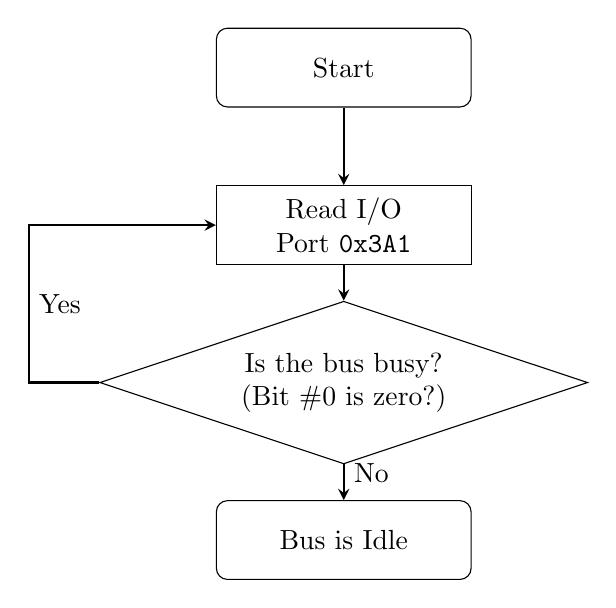
\begin{tikzpicture}[node distance=2cm]
\node (start) [startstop] {Start};
\node (read) [process, below of=start] {Read I/O Port \texttt{0x3A1}};
\node (check) [decision, below of=read] {Is the bus busy?
(Bit \#0 is zero?)};
\node (stop) [startstop, below of=check] {Bus is Idle};

\draw [arrow] (start) -- (read);
\draw [arrow] (read) -- (check);
\draw [arrow] (check) -- node[near start, anchor=west] {No} (stop);
\draw [arrow] (check) -- ++(-4cm,0) |- node[near start, anchor=west] {Yes} (read);
\end{tikzpicture}
\end{center}

\subsubsection{Transmitting Data}
To transmit data to an \itwoc{} device, complete the following sequence of operations:

\begin{center}
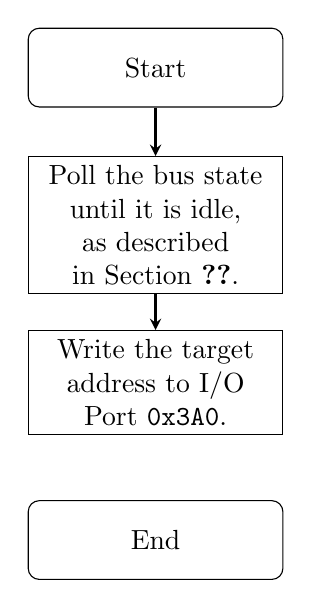
\begin{tikzpicture}[node distance=2cm]
\node (start) [startstop] {Start};
\node (waitidle1) [process, below of=start] {Poll the bus state until it is idle, as described in Section \ref{i2cbridge:busstate}.};
\node (add1) [process, below of=waitidle1] {Write the target address to I/O Port \texttt{0x3A0}.};

\node (stop) [startstop, below of=add1] {End};

\draw [arrow] (start) -- (waitidle1);
\draw [arrow] (waitidle1) -- (add1);
% \draw [arrow] (check) -- node[near start, anchor=west] {No} (stop);
% \draw [arrow] (check) -- ++(-4cm,0) |- node[near start, anchor=west] {Yes} (read);
\end{tikzpicture}
\end{center}


\begin{center}
    \begin{tabular}{ c|c|c|c|c }
        \textbf{Port} & \textbf{Direction} & \textbf{Value} & \textbf{Description} \\
        \hline
        & & & \textit{Poll the bus state until it is idle, as described in Section \ref{i2cbridge:busstate}.} \\
        \texttt{0x3A0} & W & \textit{target address} & Set the target device address. \\
        \texttt{0x3A1} & W & \texttt{0xC5} & Generate the \itwoc{} "START" condition and clock the target address on the \itwoc{} bus. \\
    \end{tabular}
\end{center}

\newpage

\section{ISA Break-out}

\subsection{Introduction}
blah

\end{document}
